\documentclass[border=2mm]{standalone}

\usepackage{fontspec}
\usepackage{unicode-math}
\usepackage{amsmath}

\usepackage{pgfplots}
\pgfplotsset{compat=1.18}
\usetikzlibrary{arrows.meta, 
  calc, 
  positioning, 
  3d,
  decorations.pathreplacing, 
  calligraphy}
\usetikzlibrary{patterns}

\usepackage{xcolor}
\definecolor{den-1}{HTML}{111111}   % Đen #111111
\definecolor{den-2}{HTML}{222222}   % Đen #222222
\definecolor{den-3}{HTML}{333333}   % Đen #333333
\definecolor{den-4}{HTML}{444444}   % Đen #444444
\definecolor{den-5}{HTML}{555555}   % Đen #555555
\definecolor{den-6}{HTML}{666666}   % Đen #666666


\begin{document}

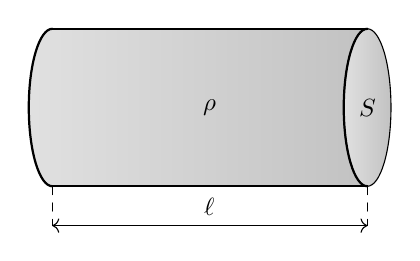
\begin{tikzpicture}[scale=1, line cap=round, line join=round]

  % Hình trụ
  \shade[left color=den-6!20, right color=den-6!40]
    (0,0) -- (4,0)
    arc[start angle=270, end angle=90, x radius=0.3, y radius=1]
    -- (0,2)
    arc[start angle=90, end angle=270, x radius=0.3, y radius=1]
    -- cycle;

  \draw[left color=den-6!20, right color=den-6!40] 
    (4,1) ellipse (0.3 and 1);
  
  % Hai đầu hình trụ
  \draw[thick] (0,0) arc[start angle=270, end angle=90, x radius=0.3, y radius=1];
  \draw[thick] (4,0) arc[start angle=270, end angle=90, x radius=0.3, y radius=1];
  \draw[thick] (0,0) -- (4,0);
  \draw[thick] (0,2) -- (4,2);

  % Viền hai đầu
  \draw[dashed] (0,0) -- ++(0,-0.5);
  \draw[dashed] (4,0) -- ++(0,-0.5);

  % Mũi tên chiều dài
  \draw[<->] (0,-0.5) -- (4,-0.5)
    node[midway, above] {\small $\ell$};

  % Nhãn bên trong
  \node at (4,1) {\small $S$};
  \node at (2,1) {\small $\rho$};

  % \shade[left color=den-6!20, right color=den-6!40] 
  %   (0,0) ellipse (0.3 and 0.8);
  
  % \shade[right color=gray!20, left color=gray!40]
  %   (0,0) -- (6,0)
  %   arc[start angle=270, end angle=90, x radius=0.3, y radius=0.8]
  %   -- (0,0);
  
  % Đầu bên phải (mặt cắt)
  % \draw[fill=gray!30] (6,0) ellipse (0.3 and 0.8);

  % Nhãn
  % \draw[<->] (0,-1.3) -- (6,-1.3) node[midway, below] {$l$};
  % \node at (3,1) {\small $\rho$};

  % Mũi tên cong và ghi chú thể tích

  % \draw [->, thick, color=den-4, rounded corners=10pt] 
  %   (2,3.5) to[bend left=30] (3.5,2.5);

  % \node at (2,3.5) [above] {\small $500\,\text{cm}^3$};

\end{tikzpicture}


\end{document}
